\documentclass{cubeamer}

\title{RBFs Over Near-Flat Surfaces}
\subtitle{APPM 5480 Asymptotics}
\author[Caleb Jacobs]{Caleb Jacobs}
\date{April 25, 2022}
\institute[University of Colorado Boulder]{Department of Applied Mathematics}
% \copyrightnotice{Published by the American Institute of Aeronautics and Astronautics, Inc., with permission}

% Useful math operators and symbols
\newcommand{\bigO}{\mathcal{O}}
\DeclareMathOperator{\sech}{sech}
\DeclareMathOperator{\csch}{csch}
\DeclareMathOperator{\arcsec}{arcsec}
\DeclareMathOperator{\arccot}{arcCot}
\DeclareMathOperator{\arccsc}{arcCsc}
\DeclareMathOperator{\arccosh}{arcCosh}
\DeclareMathOperator{\arcsinh}{arcsinh}
\DeclareMathOperator{\arctanh}{arctanh}
\DeclareMathOperator{\arcsech}{arcsech}
\DeclareMathOperator{\arccsch}{arcCsch}
\DeclareMathOperator{\arccoth}{arcCoth} 
\newcommand{\nats}{\mathbb{N}}
\newcommand{\reals}{\mathbb{R}}
\newcommand{\rats}{\mathbb{Q}}
\newcommand{\ints}{\mathbb{Z}}
\newcommand{\pols}{\mathcal{P}}
\newcommand{\cants}{\Delta\!\!\!\!\Delta}
\newcommand{\eps}{\varepsilon}
\newcommand{\st}{\backepsilon}
\newcommand{\abs}[1]{\left| #1 \right|}
\newcommand{\dom}[1]{\mathrm{dom}\left(#1\right)}
\newcommand{\for}{\text{ for }}
\newcommand{\dd}[1]{\mathrm{d}#1}
\newcommand{\spn}{\mathrm{sp}}
\newcommand{\nul}{\mathcal{N}}
\newcommand{\col}{\mathrm{col}}
\newcommand{\rank}{\mathrm{rank}}
\newcommand{\norm}[1]{\lVert #1 \rVert}
\newcommand{\inner}[1]{\left\langle #1 \right\rangle}
\newcommand{\pmat}[1]{\begin{pmatrix} #1 \end{pmatrix}}
\renewcommand{\and}{\text{ and }}

\begin{document}

\maketitle

\cutoc

\section{Introduction/Background}
\subsection{Radial Basis Functions}

\begin{frame}{Radial Basis Functions}
	A radial basis function (RBF), denoted by $ \phi(r) $, is any radially symmetric function. \pause
	\vspace{-0.25cm}
	\begin{center}
		\emph{{\small Commonly used radial basis functions}}
	\end{center}
	\vspace{-0.1cm}
	\[
		\begin{array}{ll}
			\hline
			\text{Type of basis function} & \text{Radial function } \phi(r) \\
			\hline
			\alt<3>{{\textbf{Gaussian (GA)}} & \mathbf{e^{-(\eps r)^2}}}{\text{Gaussian (GA)} & e^{-(\eps r)^2}} \\
			\text{Multiquadric(MQ)} & \sqrt{1 + (\eps r)^2} \\
			\text{Inverse Multiquadric (IMQ)} & 1 / \sqrt{1 + (\eps r)^2} \\
			\text{Inverse Quadratic (IQ)} & 1 / (1 + (\eps r)^2) \\
			\text{Sech (SH)} & \sech(\eps r)
		\end{array}
	\]
	\vspace{-0.75cm}
	where $ \eps $ is called the \emph{shape parameter} \cite{rbf}.
\end{frame}

\subsection{RBF Interpolants}

\begin{frame}{RBF Interpolants}
    Suppose we have data $ \{\mathbf{x}_i, f_i\}_{i = 1}^n $. \pause Then, we can define an RBF based interpolant as
    \[
    	s(\mathbf{x}) = \sum_{i = 1}^n \lambda_i \phi_\eps(\norm{\mathbf{x} - \mathbf{x}_i})
    \] \pause
    where $ \lambda_i $ can be found by solving
    \[
    	\underbrace{\pmat{
    			\phi_\eps (\norm{\mathbf{x}_1 - \mathbf{x}_1}) & \phi_\eps (\norm{\mathbf{x}_1 - \mathbf{x}_2}) & \cdots & \phi_\eps (\norm{\mathbf{x}_1 - \mathbf{x}_n}) \\
    			\phi_\eps (\norm{\mathbf{x}_2 - \mathbf{x}_1}) & \phi_\eps (\norm{\mathbf{x}_2 - \mathbf{x}_2}) & \cdots & \phi_\eps (\norm{\mathbf{x}_2 - \mathbf{x}_n}) \\
    			\vdots & \vdots & \ddots & \vdots \\ 
    			\phi_\eps (\norm{\mathbf{x}_n - \mathbf{x}_1}) & \phi_\eps (\norm{\mathbf{x}_n - \mathbf{x}_2}) & \cdots & \phi_\eps (\norm{\mathbf{x}_n - \mathbf{x}_n})
    	}}_{A} \underbrace{\pmat{
    			\lambda_1 \\ \lambda_2 \\ \vdots \\ \lambda_n
    	}}_{\pmb{\lambda}} = \underbrace{\pmat{
    			f_1 \\ f_2 \\ \vdots \\ f_n
    	}}_{\pmb{F}}.
    \]
\end{frame}

\subsection{Solving $ A \pmb{\lambda} = \pmb{F} $}

\begin{frame}{Solving for our weights $ \pmb{\lambda} $}
	\begin{overprint}
		\onslide<1-3>
			The smaller $ \eps $ gets, the more accurate the RBF interpolant becomes. But, as $ \eps $ becomes smaller, the conditioning of $ A $ increases.
			\begin{itemize}
				\item<2-> Naively solving $ A \pmb{\lambda} = \pmb{F} $ is called \emph{RBF-Direct}. \emph{Does not work when $ \eps $ is small.}
				\item<3-> Solve this system stably using an indirect method for small $ \eps $.
			\end{itemize}
		\onslide<4->
			So we want to use an indirect method to obtain better accuracy for small $ \eps $. \\ \onslide<5->{There is no reason for $ \eps $ to be real valued so let's leverage contour integration using Cauchy's integral formula,}
			\onslide<5->{
				\[
					\phi_\eps(x) = \frac{1}{2\pi i} \oint_\Gamma \frac{\phi_z(x)}{z - \eps} \dd z.
				\]}
			\begin{itemize}
				\item<6-> RBF Contour Pad\'e (RBF-CP) \only<7->{(\emph{precursor to RBF-RA})}
				\item<7-> RBF Rational Approximations (RBF-RA) (circa 2017) \cite{rbf-ra}
			\end{itemize}
	\end{overprint}
\end{frame}

\begin{frame}{RBF-RA issues}
	RBF-RA works great when the data given $ \{\mathbf{x}_i\}_{i = 1}^n $ is
	\begin{itemize}
		\item<1-> on a completely flat surface
		\item<1-> on a curvy surface.
	\end{itemize}
	\onslide<2->{
		However, RBF-RA breaks down when the data is on a near-flat surface (i.e. surface with small curvature).
		
		So, we would like understand/explore why RBF-RA breaks on near flat surfaces.
	}
\end{frame}


\section{Enter Asymptotics!}
\subsection{A perturbation problem}

\begin{frame}
	\frametitle{A perturbation problem}
	\begin{overprint}
		\onslide<1-2>
			Suppose we have the pairs of points $ \{(x_i, y_i)\}_{i = 1}^n $ in the \emph{unit disk}. Then, define our interpolation nodes as
			\[
				\mathbf{x}_i = \left\langle x_i, y_i, \sqrt{\frac{1}{\kappa^2} - r_i^2} - \frac{1}{\kappa}\right\rangle, \quad r_i = \sqrt{x_i^2 + y_i^2}.
			\]
			This is just data over a sphere with curvature $ \kappa $ with the top of the sphere at the origin:
			\only<1>{\vspace{-0.75cm}
				\begin{figure}[h!]
					\centering
					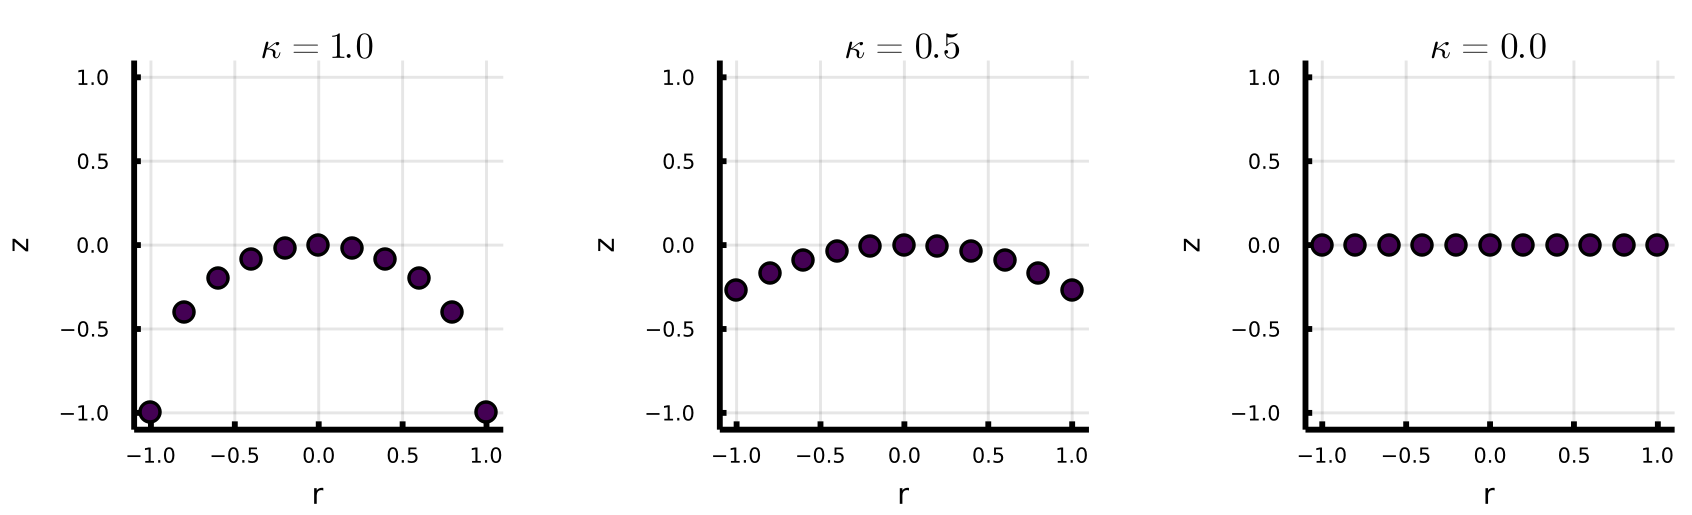
\includegraphics[width = 0.75\textwidth]{Images/Curves.png}
			\end{figure}}
			\only<2>{\[
				x_i^2 + y_i^2 + (z_i + 1 / \kappa)^2 = \frac{1}{\kappa^2}
			\]}
		\onslide<3-4>
			\[
				\mathbf{x}_i = \left\langle x_i, y_i, \sqrt{\frac{1}{\kappa^2} - r_i^2} - \frac{1}{\kappa}\right\rangle, \quad r_i = \sqrt{x_i^2 + y_i^2}.
			\]
			Then, the difference between two nodes is given as 
			\[
				\norm{\mathbf{x}_i - \mathbf{x}_j}_2^2 = (x_i - x_j)^2 + (y_i - y_j)^2 + \left(\sqrt{\frac{1}{\kappa^2} - r_i^2} - \sqrt{\frac{1}{\kappa^2} - r_j^2}\right)^2
			\]
			\onslide<4>{
				Further, each entry of the collocation matrix $ A $ will be
				\[
					A_{ij} = \phi_\eps(\norm{\mathbf{x}_i - \mathbf{x}_j}_2) = e^{-(\eps \norm{\mathbf{x}_i - \mathbf{x}_j}_2)^2} = e^{-\eps^2 \norm{\mathbf{x}_i - \mathbf{x}_j}_2^2}
				\]
			}
		\onslide<5-6>
			\begin{align*}
				A_{ij} &= \phi_\eps(\norm{\mathbf{x}_i - \mathbf{x}_j}_2) = e^{-(\eps \norm{\mathbf{x}_i - \mathbf{x}_j}_2)^2} = e^{-\eps^2 \norm{\mathbf{x}_i - \mathbf{x}_j}_2^2} \\
	          			  &= e^{-\eps^2 \left((x_i - x_j)^2 + (y_i - y_j)^2 + \left(\sqrt{\frac{1}{\kappa^2} - r_i^2} - \sqrt{\frac{1}{\kappa^2} - r_j^2}\right)^2\right)} \\
	         		      &= e^{-\eps^2((x_i - x_j)^2 + (y_i - y_j)^2)} e^{-\eps^2 \left(\sqrt{\frac{1}{\kappa^2} - r_i^2} - \sqrt{\frac{1}{\kappa^2} - r_j^2}\right)^2} \\
	          			  &= e^{-\eps^2((x_i - x_j)^2 + (y_i - y_j)^2)} \left(1 - \frac{1}{4} \eps^2 \kappa^2 (r_i^2 - r_j^2)^2 + \cdots\right) \\
	        			  &= e^{-\eps^2((x_i - x_j)^2 + (y_i - y_j)^2)} - \kappa^2 \frac{1}{4} \eps^2 (r_i^2 - r_j^2)^2 e^{-\eps^2((x_i - x_j)^2 + (y_i - y_j)^2)} + \bigO(\kappa^4).
			\end{align*}
			\onslide<6>{
				\vspace{-0.5cm}
				\[
					A = A_0 + \kappa^2 A_1 + \bigO(\kappa^4)
				\]
			}
		\onslide<7->
			With the expansion of $ A $
			\[
				A = A_0 + \kappa^2 A_1 + \cdots,
			\]
			our perturbed interpolant problem is then given by
			\[
				A\pmb{\lambda} = \pmb{F} \implies (A_0 + \kappa^2 A_1 + \cdots) \pmb{\lambda} = \pmb{F}, \quad 0 < \kappa \ll 1.
			\]
			
			\onslide<8>{
				Note, $ A_0 $ is just the standard collocation matrix if our data was on a flat surface. We know
				\begin{itemize}
					\item $ A_0 $ is nonsingular for $ \eps \in \reals, \eps \neq 0 $,
					\item $ A_0 $ is symmetric \cite{rbf},
					\item RBF-RA is able to stably work with $ A_0 $.
				\end{itemize}
			}
	\end{overprint}
\end{frame}

\subsection{Perturbed solution}

\begin{frame}
	\frametitle{Perturbed interpolation weights problem}
	\vspace{-0.5cm}
	\[
		 (A_0 + \kappa^2 A_1 + \cdots) \pmb{\lambda} = \pmb{F}, \quad 0 < \kappa \ll 1
	\]
	Assume $ \pmb{\lambda} $ has the regular expansion
	\[
		\pmb{\lambda} = \pmb{\lambda}_0 + \kappa^2 \pmb{\lambda}_1 + \cdots.
	\]
	
	\onslide<2->{
		Then at
		\begin{align*}
			\bigO(1)&:  A_0 \pmb{\lambda}_0 = \pmb{F} \implies \pmb{\lambda}_0 = A_0^{-1} \pmb{F} \\
			\bigO(\kappa^2)&: A_0 \pmb{\lambda}_1 + A_1 \pmb{\lambda}_0 = 0 \implies \pmb{\lambda}_1 = -A_0^{-1} A_1 \pmb{\lambda}_0 \\
			\bigO(\kappa^4) &: A_0 \pmb{\lambda}_2 + A_1 \pmb{\lambda}_1 + A_ 2 \pmb{\lambda}_0 = 0 \implies \pmb{\lambda}_2 = -A_0^{-1} (A_1 \pmb{\lambda}_1 + A_2 \pmb{\lambda}_0)
		\end{align*}
	}
	\onslide<3->{
		So in general, 
		\[
			\pmb{\lambda}_n = -A_0^{-1} (A_1\pmb{\lambda}_{n - 1} + A_2 \pmb{\lambda}_{n - 2} + \cdots + A_n \pmb{\lambda}_0).
		\]
	}
\end{frame}

\subsection{Solution remarks}

\begin{frame}
	\frametitle{Remarks}
	\begin{overprint}
		Putting everything together, our interpolation weights can be written as
		\begin{align*}
			\pmb{\lambda} &= \pmb{\lambda}_0 + \kappa^2 \pmb{\lambda}_1 + \cdots \\
			\pmb{\lambda}_n &= -A_0^{-1} (A_1\pmb{\lambda}_{n - 1} + A_2 \pmb{\lambda}_{n - 2} + \cdots + A_n \pmb{\lambda}_0)
		\end{align*}
		\onslide<2-3>
		\textbf{Remarks}
		\begin{itemize}
			\item<2-> This shows that $ \pmb{\lambda} $ is asymptotically well behaved when $ \kappa \to 0 $. So ideally, RBF-RA ought to not break in this limit.
			\item<3-> We can use this asymptotic expansion to bypass the small curvature issue in RBF-RA.
		\end{itemize}
		\onslide<4-5>
			\textbf{Modified RBF-RA Algorithm}
			\begin{enumerate}[label = (\alph*)]
				\item Compute $ \kappa $ estimate of data using desired algorithm
				\item Use RBF-RA to stably compute needed $ \pmb{\lambda}_i $
				\item Compute $ \pmb{\lambda} $ using $ \pmb{\lambda} = \pmb{\lambda}_0 + \kappa^2 \pmb{\lambda}_1 + \cdots $ up to desired term.
			\end{enumerate}
			\onslide<5>{
				Patching an algorithm like this is not ideal. Instead, we would like to understand why the algorithm breaks and then fix the algorithm at the fundamental level.
			}
	\end{overprint}
\end{frame}

\section{What's Next}

\begin{frame}
	\frametitle{A closer look at conditioning}
	The conditioning of the collocation matrix at various $ \kappa $ and $ \eps $ in the complex plane can be seen below
	\begin{figure}
		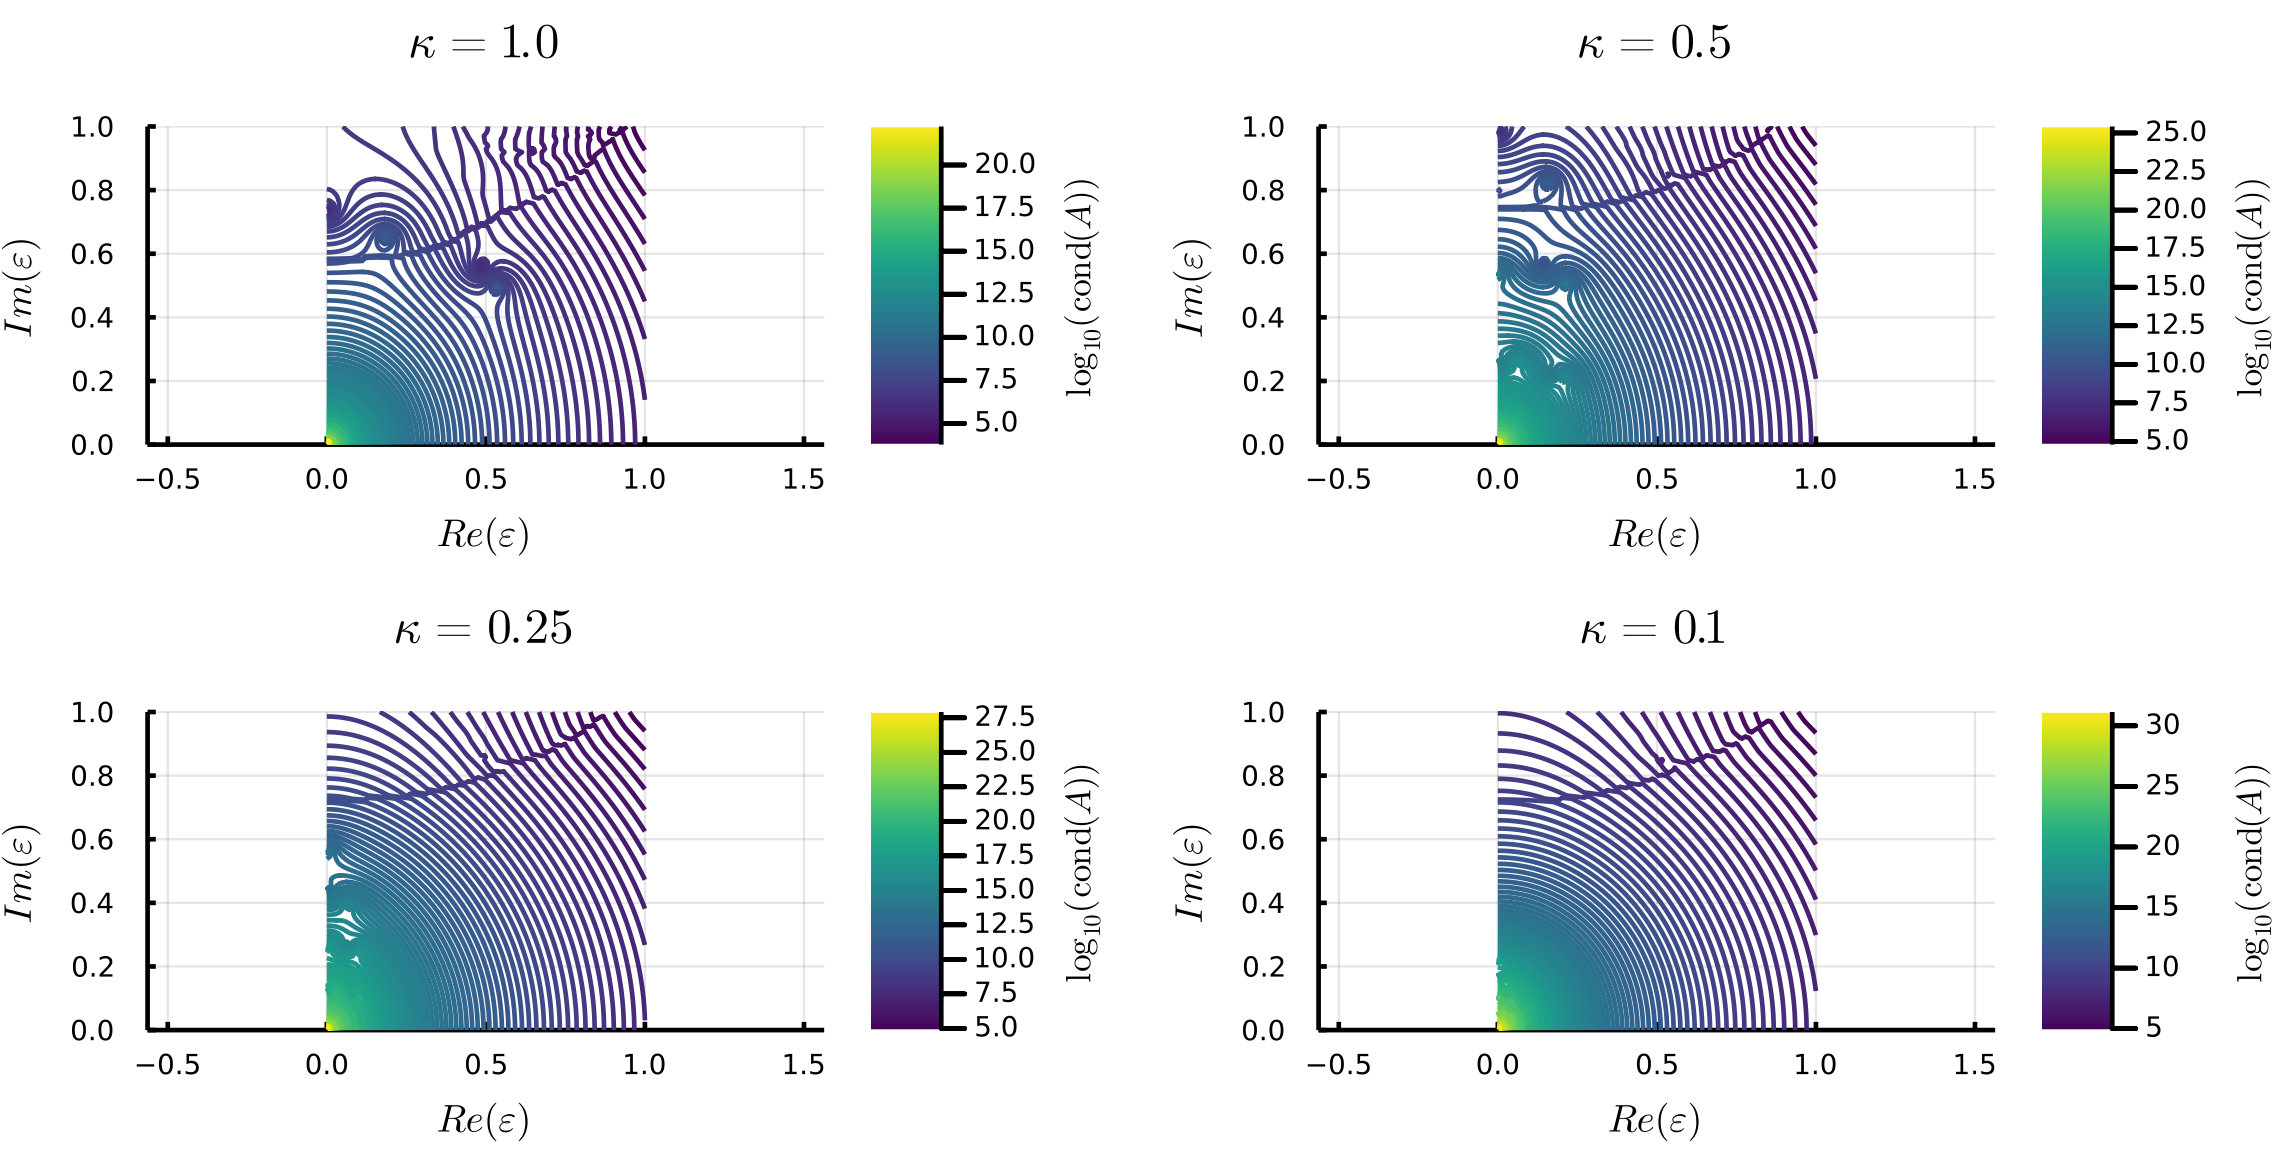
\includegraphics[width = 0.75\textwidth]{Images/Conditioning.png}
	\end{figure}
\end{frame}

\begin{frame}
	\frametitle{A perturbed eigenvalue problem}
	Using the same perturbed collocation matrix as before, we can pose a perturbed eigenvalue problem as
	\[
		(A_0 + \kappa^2 A_1 + \cdots) \mathbf{x} = \lambda \mathbf{x}. 
	\]
	Now, because $ A $ depends on arbitrary, real life data, it is reasonable to assume that $ A $ has all distinct eigenvalues. So, finding a perturbed eigenvalue/eigenvector solution to this is readily found using our formulas derived early on in our course or in $ Hinch $ \cite{hinch}. In this case, the eigenvalues all have regular perturbations
	\[
		\lambda(\eps; \kappa) = \lambda_0(\eps) + \kappa^2 \lambda_2(\eps) + \cdots.
	\]
\end{frame}

\begin{frame}
	\frametitle{A perturbed root finding problem}
	The $ A $ matrix is normal and so
	\[
		\mathrm{cond}(A) = \frac{\abs{\lambda_{\max}}}{\abs{\lambda_{\min}}}.
	\]
	So, to understand when the condition number blows up, we want to know when $ \lambda(\eps; \kappa) = 0 $ for any of the eigenvalues $ \lambda $. So, an interesting perturbed root finding problem is find $ \eps $ such that
	\[
		\lambda_0(\eps) + \kappa^2 \lambda_2(\eps) + \cdots = 0, \quad 0 < \kappa \ll 1.
	\]
	Even  for simple node-sets, $ \lambda_i(\eps) $ can be very nonlinear making this perturbed root finding problem quite difficult.
	
\end{frame}

\begin{frame}
	\frametitle{References}
	\bibliographystyle{siam}
	\bibliography{bib}
\end{frame}

\begin{frame}[standout]
    \Huge\textsc{Thank You}
    
    \vfill
    
    \LARGE\textsc{Any questions?}
\end{frame}

\end{document}

